\subsubsection{Thin scintillator cosmic ray method}
\label{sect:Thin_scintillator}

Another method of counter resolution determination is so-called "thin scintillator cosmic rays method" that uses two thin scintillators to effectively collimate cosmic rays
trajectories to perpendicularly traverse the counter at a fixed position, as shown in Fig.$\:$\ref{fig:thin_method1}. In this method time information from top and bottom counters is not needed. In order to fix track position signal coincidence  in six PMTs is required. This method was tested using five millimeters thin scintillators and it turned out that event rate is extremely low. Moreover, like in source method described in Sec.~\ref{sect:Source_method} huge amount of manual measurements is needed. 

\begin{figure}[]
\centering
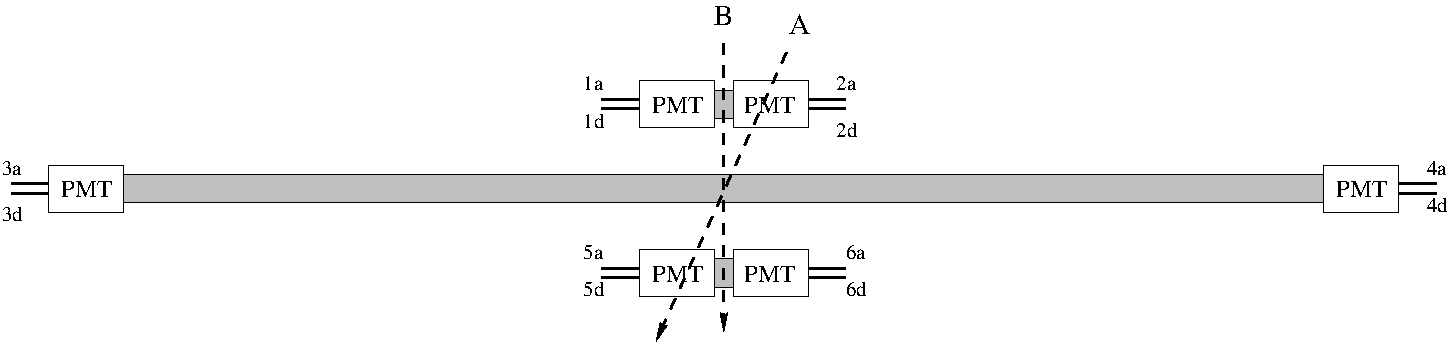
\includegraphics[width=0.9\textwidth]{gleb/fig_gleb_thin_scintillator/thin_method1.pdf}
\caption{In the thin scintillator cosmic ray  method, 5mm-thin scintillators are placed above and below the
counter to be tested so that the position of cosmic ray events on the middle counter is fixed. The
TDC difference between left and right PMTs on the middle counter is then used to determine the
counter's resolution. Only vertical tracks such as B survive, when signals in six PMTs are in coincidence. \label{fig:thin_method1}}
\end{figure}

In order to increase event rate this method can be modified as shown in Fig.$\:$\ref{fig:thin_method2}. In that case one thin scintillator ten times thicker than in previous setup is positioned between two longer scintillators achieving a partial collimation. Since non vertical tracks shown as A on Fig.$\:$\ref{fig:thin_method2} pass only part of the middle scintillator height, amplitudes of their signals are lower  then from the vertical tracks shown by B on Fig.$\:$\ref{fig:thin_method2}. So the positions on top and bottom scintillators are further restricted by cutting away low ADC events on the middle bar. But it turned out that this procedure does not sufficiently increase event rate and does not allow to get rid of the multiple manual measurements.




\begin{figure}[]
\centering
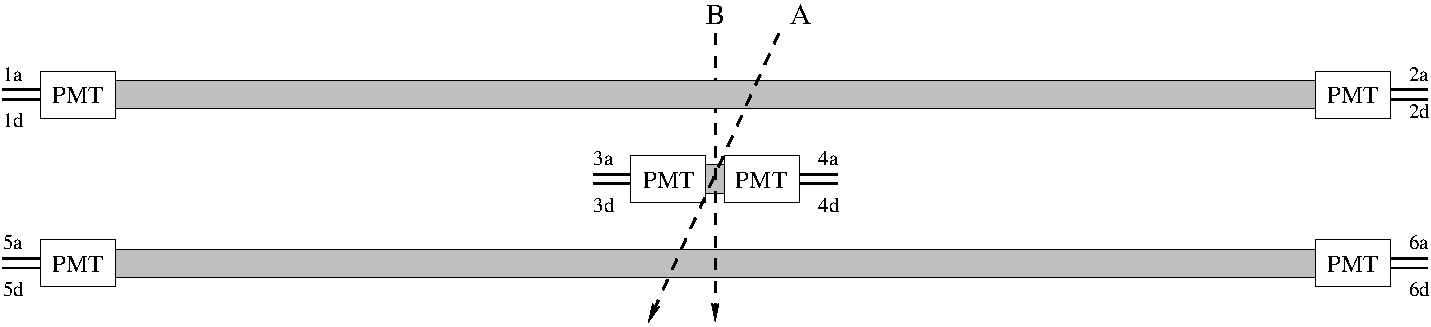
\includegraphics[width=0.9\textwidth]{gleb/fig_gleb_thin_scintillator/thin_method2.pdf}
\caption{This variant of the reference counter method does not physically restrict particles to pass
through vertically (path B), because particles along path A also triggers all six PMTs. However,
paths such as A are further reduced by cutting away middle-bar low ADC values, which correspond
generally to particles traveling through less than the 5-cm vertical extent of the middle scintillator.\label{fig:thin_method2}}
\end{figure}


Both described variants of thin scintillator cosmic rays method can be transformed into so-called "reference counter method", in which thin scintillator counters need to be replaced by reference counters with known resolutions. In that case one should use TDC information from reference counters and vertical tracks selection is not needed anymore that lead to the higher event rate. Then it becomes possible for setup like shown on Fig.$\:$\ref{fig:thin_method1} to derive the resolution of tested counter through the resulutions of reference counters, and for setup like shown on Fig.$\:$\ref{fig:thin_method2}  to derive the combined resolution of two tested counters through the resolution of the known one. 

In case of the need to test many similar counters it is natural to build setup from the three counters of the same lenght and to extract their combined resolution. These modifications lead to the three bar cosmic rays method described in Sec.~\ref{sect:Three_Bar_Cosmic_Ray_Method}
